\documentclass[14pt]{extbook}
\usepackage{multicol, enumerate, enumitem, hyperref, color, soul, setspace, parskip, fancyhdr} %General Packages
\usepackage{amssymb, amsthm, amsmath, latexsym, units, mathtools} %Math Packages
\everymath{\displaystyle} %All math in Display Style
% Packages with additional options
\usepackage[headsep=0.5cm,headheight=12pt, left=1 in,right= 1 in,top= 1 in,bottom= 1 in]{geometry}
\usepackage[usenames,dvipsnames]{xcolor}
\usepackage{dashrule}  % Package to use the command below to create lines between items
\newcommand{\litem}[1]{\item#1\hspace*{-1cm}\rule{\textwidth}{0.4pt}}
\pagestyle{fancy}
\lhead{Progress Quiz 6}
\chead{}
\rhead{Version B}
\lfoot{9689-6866}
\cfoot{}
\rfoot{Spring 2021}
\begin{document}

\begin{enumerate}
\litem{
Construct the lowest-degree polynomial given the zeros below. Then, choose the intervals that contain the coefficients of the polynomial in the form $ax^3+bx^2+cx+d$.\[ \frac{5}{2}, 4, \text{ and } \frac{7}{2} \]\begin{enumerate}[label=\Alph*.]
\item \( a \in [-1, 6], b \in [36, 45], c \in [129, 132], \text{ and } d \in [133, 144] \)
\item \( a \in [-1, 6], b \in [7, 14], c \in [-52, -45], \text{ and } d \in [-143, -137] \)
\item \( a \in [-1, 6], b \in [-48, -32], c \in [129, 132], \text{ and } d \in [133, 144] \)
\item \( a \in [-1, 6], b \in [-26, -19], c \in [-27, -17], \text{ and } d \in [133, 144] \)
\item \( a \in [-1, 6], b \in [-48, -32], c \in [129, 132], \text{ and } d \in [-143, -137] \)

\end{enumerate} }
\litem{
Describe the zero behavior of the zero $x = 9$ of the polynomial below.\[ f(x) = 7(x + 8)^{8}(x - 8)^{7}(x + 9)^{12}(x - 9)^{7} \]\begin{enumerate}[label=\Alph*.]
\begin{multicols}{2}\item 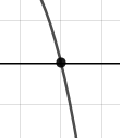
\includegraphics[width = 0.3\textwidth]{../Figures/polyZeroBehaviorAB.png}\item 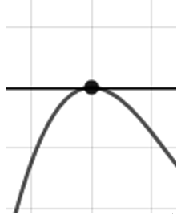
\includegraphics[width = 0.3\textwidth]{../Figures/polyZeroBehaviorBB.png}\item 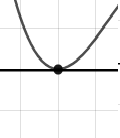
\includegraphics[width = 0.3\textwidth]{../Figures/polyZeroBehaviorCB.png}\item 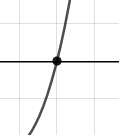
\includegraphics[width = 0.3\textwidth]{../Figures/polyZeroBehaviorDB.png}\end{multicols}\item None of the above.
\end{enumerate} }
\litem{
Which of the following equations \textit{could} be of the graph presented below?
\begin{center}
    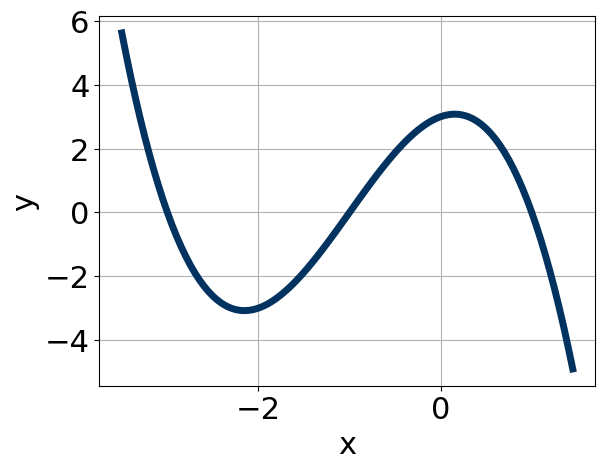
\includegraphics[width=0.5\textwidth]{../Figures/polyGraphToFunctionB.png}
\end{center}
\begin{enumerate}[label=\Alph*.]
\item \( -4(x - 3)^{6} (x + 3)^{8} (x - 2)^{7} \)
\item \( -11(x - 3)^{4} (x + 3)^{10} (x - 2)^{8} \)
\item \( 6(x - 3)^{4} (x + 3)^{9} (x - 2)^{9} \)
\item \( 6(x - 3)^{6} (x + 3)^{8} (x - 2)^{8} \)
\item \( 19(x - 3)^{8} (x + 3)^{10} (x - 2)^{7} \)

\end{enumerate} }
\litem{
Describe the zero behavior of the zero $x = 9$ of the polynomial below.\[ f(x) = -4(x + 9)^{9}(x - 9)^{10}(x - 2)^{7}(x + 2)^{10} \]\begin{enumerate}[label=\Alph*.]
\begin{multicols}{2}\item 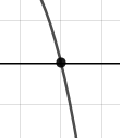
\includegraphics[width = 0.3\textwidth]{../Figures/polyZeroBehaviorCopyAB.png}\item 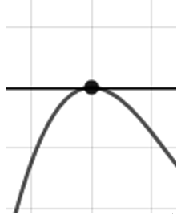
\includegraphics[width = 0.3\textwidth]{../Figures/polyZeroBehaviorCopyBB.png}\item 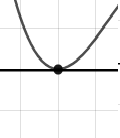
\includegraphics[width = 0.3\textwidth]{../Figures/polyZeroBehaviorCopyCB.png}\item 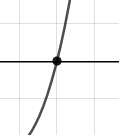
\includegraphics[width = 0.3\textwidth]{../Figures/polyZeroBehaviorCopyDB.png}\end{multicols}\item None of the above.
\end{enumerate} }
\litem{
Which of the following equations \textit{could} be of the graph presented below?
\begin{center}
    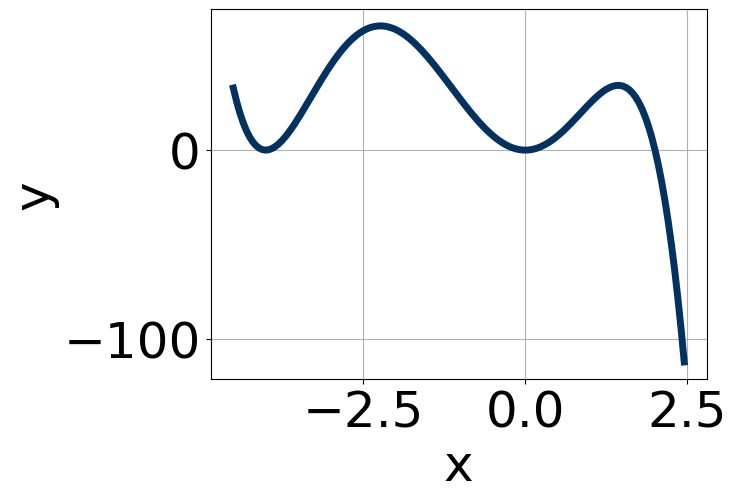
\includegraphics[width=0.5\textwidth]{../Figures/polyGraphToFunctionCopyB.png}
\end{center}
\begin{enumerate}[label=\Alph*.]
\item \( -12x^{9} (x - 2)^{5} (x - 1)^{11} \)
\item \( 18x^{4} (x - 2)^{6} (x - 1)^{11} \)
\item \( 10x^{10} (x - 2)^{5} (x - 1)^{11} \)
\item \( -10x^{6} (x - 2)^{11} (x - 1)^{9} \)
\item \( 12x^{11} (x - 2)^{11} (x - 1)^{11} \)

\end{enumerate} }
\litem{
Describe the end behavior of the polynomial below.\[ f(x) = -9(x + 9)^{2}(x - 9)^{3}(x + 7)^{2}(x - 7)^{2} \]\begin{enumerate}[label=\Alph*.]
\begin{multicols}{2}\item 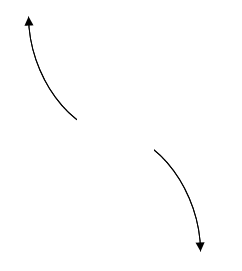
\includegraphics[width = 0.3\textwidth]{../Figures/polyEndBehaviorCopyAB.png}\item 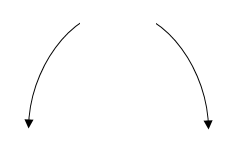
\includegraphics[width = 0.3\textwidth]{../Figures/polyEndBehaviorCopyBB.png}\item 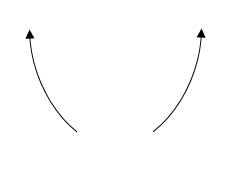
\includegraphics[width = 0.3\textwidth]{../Figures/polyEndBehaviorCopyCB.png}\item 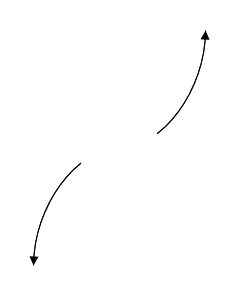
\includegraphics[width = 0.3\textwidth]{../Figures/polyEndBehaviorCopyDB.png}\end{multicols}\item None of the above.
\end{enumerate} }
\litem{
Construct the lowest-degree polynomial given the zeros below. Then, choose the intervals that contain the coefficients of the polynomial in the form $x^3+bx^2+cx+d$.\[ -3 - 5 i \text{ and } 1 \]\begin{enumerate}[label=\Alph*.]
\item \( b \in [-6.1, -3.5], c \in [26.18, 29.01], \text{ and } d \in [32.07, 34.51] \)
\item \( b \in [0.1, 4.8], c \in [0.84, 2.43], \text{ and } d \in [-3.52, -2.55] \)
\item \( b \in [3.2, 10.8], c \in [26.18, 29.01], \text{ and } d \in [-35.08, -33.01] \)
\item \( b \in [0.1, 4.8], c \in [3.67, 5.55], \text{ and } d \in [-5.68, -3.99] \)
\item \( \text{None of the above.} \)

\end{enumerate} }
\litem{
Describe the end behavior of the polynomial below.\[ f(x) = 3(x - 6)^{4}(x + 6)^{7}(x - 5)^{2}(x + 5)^{2} \]\begin{enumerate}[label=\Alph*.]
\begin{multicols}{2}\item 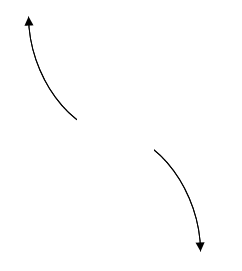
\includegraphics[width = 0.3\textwidth]{../Figures/polyEndBehaviorAB.png}\item 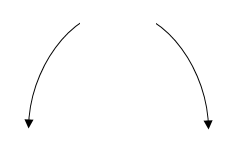
\includegraphics[width = 0.3\textwidth]{../Figures/polyEndBehaviorBB.png}\item 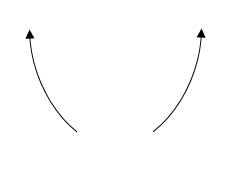
\includegraphics[width = 0.3\textwidth]{../Figures/polyEndBehaviorCB.png}\item 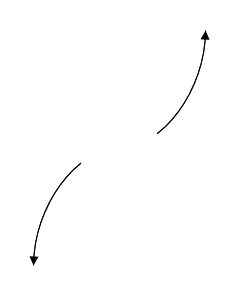
\includegraphics[width = 0.3\textwidth]{../Figures/polyEndBehaviorDB.png}\end{multicols}\item None of the above.
\end{enumerate} }
\litem{
Construct the lowest-degree polynomial given the zeros below. Then, choose the intervals that contain the coefficients of the polynomial in the form $x^3+bx^2+cx+d$.\[ 4 - 4 i \text{ and } 1 \]\begin{enumerate}[label=\Alph*.]
\item \( b \in [5, 10], c \in [31, 46], \text{ and } d \in [24, 34] \)
\item \( b \in [1, 2], c \in [-10, -1], \text{ and } d \in [3, 12] \)
\item \( b \in [-14, -8], c \in [31, 46], \text{ and } d \in [-34, -30] \)
\item \( b \in [1, 2], c \in [3, 4], \text{ and } d \in [-5, 0] \)
\item \( \text{None of the above.} \)

\end{enumerate} }
\litem{
Construct the lowest-degree polynomial given the zeros below. Then, choose the intervals that contain the coefficients of the polynomial in the form $ax^3+bx^2+cx+d$.\[ \frac{1}{4}, -5, \text{ and } \frac{-7}{5} \]\begin{enumerate}[label=\Alph*.]
\item \( a \in [17, 24], b \in [-128, -121], c \in [108, 114], \text{ and } d \in [32, 38] \)
\item \( a \in [17, 24], b \in [132, 140], c \in [166, 173], \text{ and } d \in [32, 38] \)
\item \( a \in [17, 24], b \in [118, 125], c \in [108, 114], \text{ and } d \in [32, 38] \)
\item \( a \in [17, 24], b \in [118, 125], c \in [108, 114], \text{ and } d \in [-42, -31] \)
\item \( a \in [17, 24], b \in [-70, -65], c \in [-163, -155], \text{ and } d \in [-42, -31] \)

\end{enumerate} }
\end{enumerate}

\end{document}